\clearpage
\section{Simulation Analysis}
\label{sec:simulation}

\subsection{Step 1}

Table~\ref{tab:op1} shows the simulated operating point results for the circuit
under analysis, for $t<0$. 


\subsection{Step 2}

Table~\ref{tab:op2} shows the simulated operating point results for the circuit
under analysis, for $t=0$. 

Here, $I_x = -vx\#branch$ because it is not possible to define the current through the voltage source $V_x$ as going from the node n- to the node n+. It may seems that there is current through all the branches and voltages in most of the nodes, but, after observing and considering that the values given by the ``datagen'' file, they have precision till $10^{-11}$, therefore it is possible to say that voltages lesser $10^{-11} V$ and currents lesser than $10^{-11} A$ are indistinguishable from 0.\\


\begin{minipage}[b]{0.46\textwidth}
\centering
   \begin{tabular}{|l|r|}
    \hline    
    {\bf Name} & {\bf Value [A or V]} \\ \hline
    \input{../sim/op1_tab}
   \end{tabular}
    \captionsetup{type=table}   
  \caption{Operating point. A variable preceded by @ or has \# in its name is of type {\em current}
    and expressed in Ampere; other variables are of type {\it voltage} and expressed in
    Volt.}
  \label{tab:op1}
\end{minipage}
\hfill
\begin{minipage}[b]{0.46\textwidth}
\centering
  \begin{tabular}{|l|r|}
    \hline    
    {\bf Name} & {\bf Value [A or V]} \\ \hline
    \input{../sim/op2_tab}
  \end{tabular}
    \captionsetup{type=table}   
  \caption{Operating point. A variable preceded by @ or has \# in its name is of type {\em current}
    and expressed in Ampere; other variables are of type {\it voltage} and expressed in
    Volt.}
  \label{tab:op2}
\end{minipage}


\clearpage
\subsection{Step 3}

Using as initial condition $V_s=0V$ and $V_c = V_6-V_8$, it was possible to simulate the natural response in the node 6, $v_{6n}(t)$. The plot can be seen in Figure~\ref{fig:sim-v6n}, for $t\in [0,20]ms$.

\begin{figure}[ht!]
    \centering
    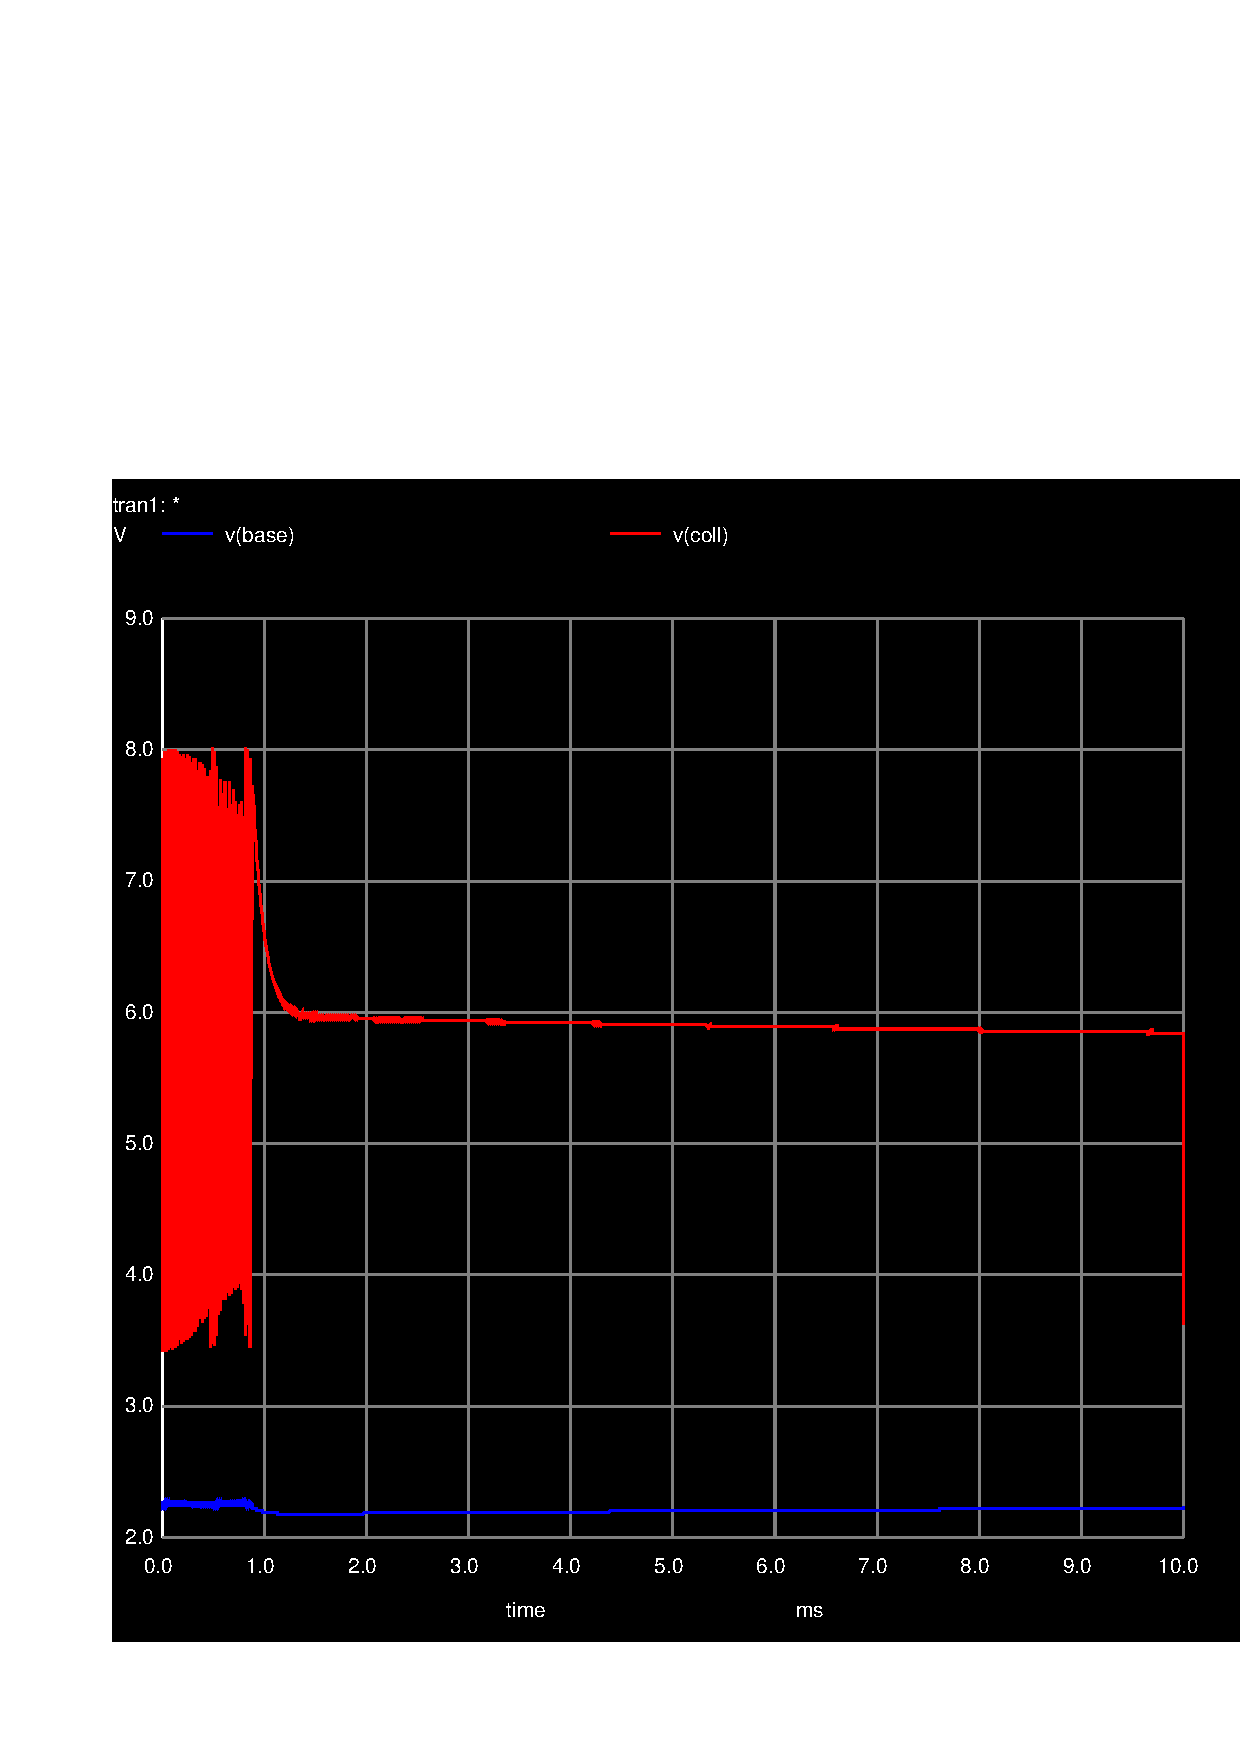
\includegraphics[width=0.5\textwidth, trim={1.8cm 2cm 0 8.1cm}]{../sim/trans.pdf}
    \caption{Natural response in node 6, for $t\in [0,20]ms$.}
    \label{fig:sim-v6n}
\end{figure}
\FloatBarrier




\subsection{Step 4}
Repeating the previous step to simulate the total response on node 6, considering $v_s(t)=~\sin(2 \pi f t)$ and frequency $f=1 kHz$. The plot containing the stimulus and the response can be seen in Figure~\ref{fig:sim-v6total}.

\begin{figure}[ht!]
    \centering
    \includegraphics[width=0.5\textwidth, trim={1.8cm 2cm 0 8.1cm}]{../sim/acdc.pdf}
    \caption{Total response in node 6, for $t\in [0,20]ms$ and $f=1 kHz$.}
    \label{fig:sim-v6total}
\end{figure}
\FloatBarrier



\subsection{Step 5}

\subsubsection{Magnitude Response}

Figure~\ref{fig:sim-db} shows the magnitude of the frequency response for the
circuit under analysis, for the voltages $v_c(f),\ v_6(f)$ and $v_s(f)$, with $f$ from 0.1 \textit{Hz} to 1 \textit{MHz}.

\begin{figure}[ht!] \centering
\includegraphics[width=0.5\linewidth, trim={1.8cm 2cm 0 8.1cm}]{../sim/sim-db.pdf}
\caption{Magnitude response.}
\label{fig:sim-db}
\end{figure}
\FloatBarrier


\subsubsection{Phase Response}

Figure~\ref{fig:sim-phase} shows the phase in degrees of the frequency response for the
circuit under analysis.

\begin{figure}[ht!] \centering
\includegraphics[width=0.5\linewidth, trim={1.8cm 2cm 0 8.1cm}]{sim-phase.pdf}
\caption{Phase response.}
\label{fig:sim-phase}
\end{figure}
\FloatBarrier
